\documentclass[]{article}

\usepackage{graphicx} % dvips destroys the tikzpicture to a mess

\usepackage{tikz}
\usetikzlibrary{shapes.geometric,arrows}
%
\tikzstyle{startstop} = [rectangle, rounded corners, text centered, draw=black, fill=blue!10]
\tikzstyle{process} = [rectangle, minimum width=2cm, minimum height=1cm, text centered, draw=black, fill=orange!10]
\tikzstyle{decision} = [diamond, aspect=3, minimum width=3cm, minimum height=1cm, text centered, draw=black, fill=red!10]
% define arrow style
\tikzstyle{compute} = [rectangle, minimum width=2cm, minimum height=1cm, text centered, draw=black, fill=green!10]
\tikzstyle{estimate} = [rectangle, rounded corners, minimum width=2cm, minimum height=1cm, text centered, draw=black, fill=yellow!10]
\tikzstyle{arrow} = [thick,->,>=stealth]

\begin{document}

\begin{figure}\centering 
	%the \par is necessary after each text to make the \baselineskip take effect
	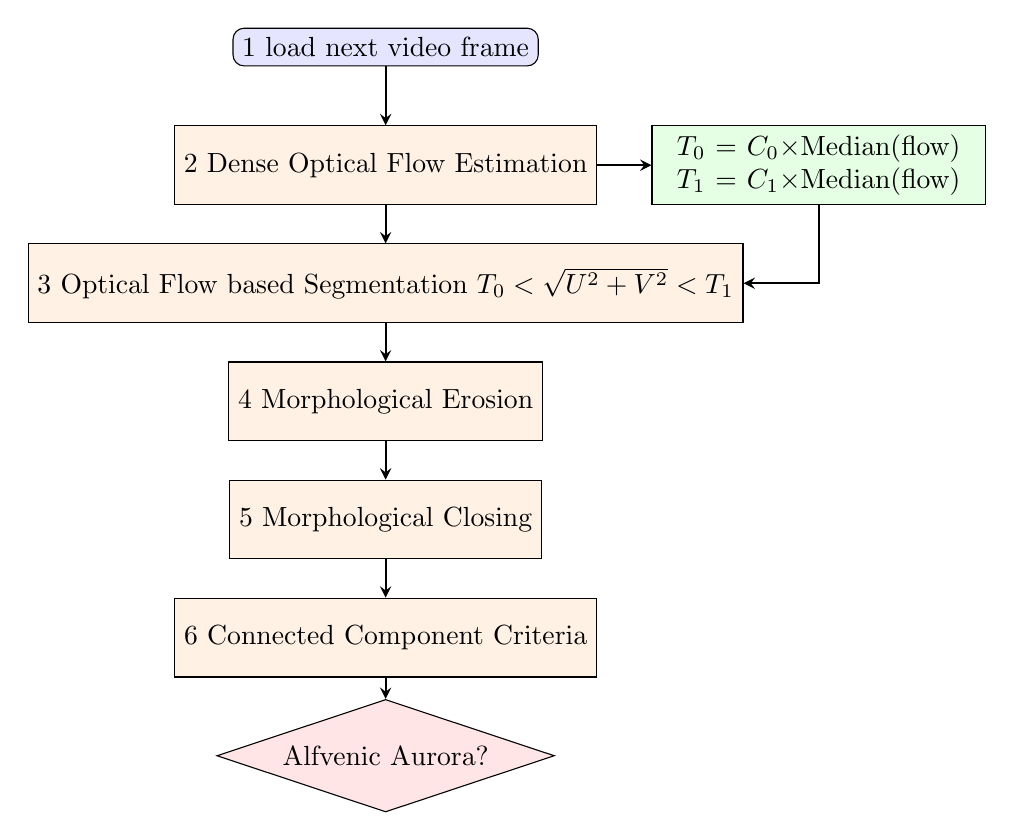
\begin{tikzpicture}[node distance=1.5cm, auto]
	
	\node (in) [startstop] {1 load next video frame \par};
	
	\node (flow) [process, below of=in] {2 Dense Optical Flow Estimation \par };
	
	\node (med) [compute, right of=flow,xshift=4cm, text width=4cm] { $T_0 = C_0 \times$Median(flow) $T_1 = C_1 \times$Median(flow) \par };
	
	\node (seg) [process, below of=flow]{3 Optical Flow based Segmentation $ T_0 < \sqrt{U^2 + V^2} < T_1 $ \par};
	
	\node (erode) [process, below of=seg]{4 Morphological Erosion \par};
	
	\node (close) [process, below of=erode]{5 Morphological Closing \par};
	
	\node (blob) [process, below of=close]{6 Connected Component Criteria \par};
	
	\node(detect) [decision, below of=blob]{Alfvenic Aurora? \par};
	
	%
	

	\draw[arrow] (in) -- (flow);
	\draw[arrow] (flow) -- (med);
	\draw[arrow] (med) |- (seg);
	\draw[arrow] (flow) -- (seg);
	\draw[arrow] (seg) -- (erode);
	\draw[arrow] (erode) -- (close);
	\draw[arrow] (close) -- (blob);
	\draw[arrow] (blob) -- (detect);
	
	\end{tikzpicture}
	
	\caption{Block diagram of Alfvenic aurora detection algorithm.}
	\label{fig:blockcv}
\end{figure}

\end{document}